\documentclass[12pt]{article}

\usepackage[utf8]{inputenc}
\usepackage[spanish]{babel}
\usepackage[dvipsnames]{xcolor}
\usepackage{amssymb}
\usepackage{physics}
\usepackage{amsmath}
\usepackage{anysize}
\usepackage{multicol} 
\usepackage{graphicx}                      
\usepackage{blindtext}                                          
\usepackage{cancel}
\usepackage{tikz}
\usepackage[square,numbers]{natbib}

\usepackage{hyperref}
 \hypersetup{ colorlinks = true, linkcolor = black } %==== Hipervínculos ====%
\usepackage{geometry}
\newgeometry{ bottom = 2.54cm, top = 2.54cm, left = 2.54cm, right = 2.54cm } %==== Modificación de Márgenes ====%

\usepackage{fancyhdr}  
\pagestyle{fancy}
\fancyhf{}
\fancyhead[R]{Mecánica Clásica}
\fancyhead[L]{\thepage}
\renewcommand{\headrulewidth}{0.08pt} %==== Encabezados ====%

\renewcommand{\footrulewidth}{0.08pt} %==== Pie de Página ====%
\fancyfoot[L]{}
\fancyfoot[R]{\rightmark}

%\usepackage[pages=all]{background} 
%\backgroundsetup{ scale=1, color=black, opacity=0.15, angle=0,
 %   contents={ 
\includegraphics{logo_ifuap.png} }
%}

\setcounter{tocdepth}{3}

\newcommand{\Title}[1]{\begin{center} \LARGE{\textbf{\textit{#1}}} \end{center}}
\newcommand{\Abstract}[1]{\begin{abstract} \normalsize{#1} \end{abstract}}
\newcommand{\Theorem}[1]{\begin{center} \normalsize{\textit{#1}} \end{center}}

\newcommand{\blue}  { \color{blue} }
\newcommand{\red}   { \color{red} }
\newcommand{\green} { \color{OliveGreen} }
\newcommand{\orange}{ \color{orange} }

\newcommand{\deq}{:=}
\newcommand{\less}{<}
\newcommand{\grow}{>}

\newcommand{\Identity}{\mathbb{I}}
\newcommand{\Reals}{\mathbb{R}}
\newcommand{\Naturals}{\mathbb{N}}
\newcommand{\Integers}{\mathbb{Z}}
\newcommand{\Complex}{\mathbb{C}}
\newcommand{\Imaginaries}{\mathbb{I}}

\newcommand{\Lag}{\mathcal{L}}
\newcommand{\Ham}{\mathcal{H}}

\newcommand{\cbk}[1]{ \left( #1 \right) }
\newcommand{\sbk}[1]{ \left[ #1 \right] }
\newcommand{\kbk}[1]{ \left\{ #1 \right\} }
\newcommand{\tbk}[1]{ \langle #1 \rangle }

\newcommand{\Grad}{ \vec{\nabla} }
\newcommand{\Divg}{ \vec{\nabla} \cdot }
\newcommand{\Curl}{ \vec{\nabla} \times }
\newcommand{\Lapl}{ \nabla^{2} }

\newcommand{\rad}[1]{ \vec{r}_{#1} }

\newcommand{\define}[3]{ \left. #1 \right|_{#2}^{#3} }
\newcommand{\Sum}[3]{ \sum_{#1=#2}^{#3} }
\newcommand{\Tensor}[3]{ #1^{#2}_{#3} }

\newcommand{\Partial}[2]{ \frac{\partial#1}{\partial#2} }
\newcommand{\SecPartial}[3]{ \frac{\partial^{2}#1}{\partial#2\partial#3} }

\newcommand{\eqLagrange}[1]{ \frac{d}{dt}\cbk{\Partial[\dot{#1}]{\Lag}} - \Partial[#1]{\Lag} = 0 }

\newcommand{\eqHamilton}[2]{ \Partial[#1_{i}]{\Ham} = - \dot{#2}_{i}, ~ ~ \Partial[#2_{i}]{\Ham} = \dot{#1}_{i} }

\begin{document}

	\Title{Evoluci\'on de un rasgo cuantitativo en una poblaci\'on monom\'orfica, enfoque con formalismo de Hamilton-Jacobi.}

	\Abstract{Reproducimos parte de los resultados expuestos en el articulo \citep{dieckman2005}, enfoc\'andonos en la evoluci\'on de un rasgo cuantitativo de una poblaci\'on monom\'orfica, y obteniendo resultados con un nuevo enfoque sobre las ecuaciones de selecci\'on-mutaci\'on utilizadas, en este caso con el formalismo de Hamilton-Jacobi.}
	\tableofcontents
	\clearpage
%-----------------------------------------------------------------
	\section{¿Qué es la Dinámica Adaptativa?}{

        \subsection{Adaptación y Evolución de los Sistemas Biológicos.}{

            \normalsize{En el estudio de los sistemas biológicos, los conceptos de adaptación y evolución son fundamentales para comprender cómo los organismos responden a su entorno y cómo estas respuestas moldean la diversidad de la vida en la Tierra. \citep{adaptacion} La adaptación se refiere al proceso mediante el cual los organismos desarrollan características que mejoran su capacidad para sobrevivir y reproducirse en condiciones ambientales específicas. Estas características pueden ser de naturaleza física, como la presencia de pelaje grueso en animales que habitan regiones frías; fisiológica, como la capacidad de las plantas desérticas para retener agua; o conductual, como la migración estacional de las aves. La adaptación resulta principalmente de la selección natural, un mecanismo que favorece aquellas variaciones genéticas que proporcionan ventajas competitivas en un entorno particular.}\\

            \normalsize{\citep {evolucion} Por otro lado, la evolución es un proceso a largo plazo que describe los cambios genéticos acumulativos en las poblaciones de organismos a lo largo de generaciones. Este fenómeno, impulsado por la selección natural, las mutaciones genéticas, la deriva genética y el flujo génico, es responsable de la aparición de nuevas especies y de la vasta diversidad de formas de vida observada hoy en día. La evolución permite entender cómo los organismos han cambiado con el tiempo para adaptarse a condiciones ambientales cambiantes, y cómo estos cambios han contribuido al desarrollo de estructuras, comportamientos y funciones altamente especializadas.}\\

            \normalsize{La relación entre adaptación y evolución es íntima y complementaria. Mientras que la adaptación representa la respuesta inmediata de un organismo o una población a presiones selectivas específicas, la evolución engloba los cambios genéticos a largo plazo que consolidan estas adaptaciones en las poblaciones. Por ejemplo, el cuello largo de las jirafas modernas es el resultado de un proceso evolutivo que tuvo su origen en la ventaja adaptativa de alcanzar las hojas altas de los árboles en entornos de escasez alimentaria.}\\

            \normalsize{\citep{Mirrahimi} Desde la década de 1980, el término \textit{evolución adaptativa} se ha acuñado para describir los formalismos matemáticos que abordan la selección y evolución de un rasgo en una población estructurada por un rasgo fenotípico continuo. Dichos modelos se basan en tres principios fundamentales que sustentan la evolución Darwineana:}
            
                \begin{itemize}
                    \item {
                    
                        \normalsize{La multiplicación de la población.}

                    }
                    
                    \item {
                    
                        \normalsize{La selección mediante competencia por los recursos disponibles.}
                    }
                    
                    \item {
                    
                        \normalsize{Mutaciones.}

                    }
                \end{itemize}
                
            \normalsize{Modelos simples basados en estos principios pueden explicar como emergen rasgos mas aptos y, a su vez, como poblaciones caracterizadas por varios rasgos bien diferenciados pueden coexistir potencialmente. Las simulaciones numéricas pueden presentar la aparición de ciclos y la especiacion, esto debido a que los recursos limitados generan competencia; los individuos con características similares utilizan resucursos similares, dando asi, una competencia mayor entre ellos. La cuestión de comprender cómo, en un población de este tipo, una especie mutante puede invadir o no una población inicial. En modelos de población cerrada, las mutaciones forman parte de la dinámica y se toman en cuenta la heredad de los rasgos ligeramente diferente a los progenitores.}
        }
        
        \subsection{Motivación para Introducir la Teoría de Hamilton-Jacobi.}

            \normalsize{\citep{Barles2006} Las ecuaiones de Hamilton-Jacobi son herramientas útiles para describir diversas asintósitcas singulares, es decir, situaciones en las que el comportamiento de un sistema físico o matemático cambia  de manera abrupta o presenta características extremas en ciertas condiciones, como cerca de puntos críticos, bordes o zonas donde se manifiestan discontinuidades. Estas presentan soluciones límite o aproximadas en condiciones extremas.
            }\\

            \normalsize{En los sistemas ecológicos y biológicos, la adaptación y evolución son procesos fundamentales que determinan la dinámica y supervivencia de las poblaciones. La capacidad de las especies para adaptarse a cambios en su entorno a través de la selección natural, la mutación y la competencia es un tema central en biología teórica. Para modelar estos procesos, las ecuaciones de Hamilton-Jacobi (H-J) han emergido como herramientas matemáticas poderosas para describir la evolución de poblaciones bajo distintos escenarios ecológicos.}\\

            \normalsize{\citep{Nicolas} La ecuación de Hamilton-Jacobi encuentra su aplicación en sistemas donde la dinámica de selección-mutación desempeña un papel clave. En este contexto, el cambio en el tiempo del valor de una cierta característica $\hat{s}$ en una población monomórfica, se da por medio de una ecuación de selección-mutación:}

            \begin{equation*}
                \frac{d \hat{s}}{d t}=\mu(\hat{s}) \frac{\sigma_0^2(\hat{s})}{2} n(\hat{s}) \partial_1 f(\hat{s}, \hat{s})
            \end{equation*}

            \normalsize{donde $\mu(s)$ es la probabilidad de que un nacimiento de un individuo con una característica $\hat{s}$ surja de una mutación; $\sigma_0^2(s)$ denota la varianza de distribución de una mutación $\hat{s'}$ proveniente de un individuo con característica $\hat{s}$; $\partial_1 f(\hat{s}, \hat{s}$ representa los parametros de intereacción entre individuos con característica $\hat{s}$ y $\hat{s'}$ dado por la natalidad y mortandad.}\\

            \normalsize{\citep{Calves} En el límite donde la tasa de mutación \( \mu \) es pequeña, las densidades de población tienden a concentrarse alrededor de valores particulares de \( x \), representando adaptaciones específicas. Este comportamiento puede analizarse mediante un ansatz de la forma:}

            \begin{equation*}
                u(x, t) \sim e^{\varphi(x, t)/\mu}
            \end{equation*}
                
            \normalsize{donde $\varphi(x,t)$ representa el frente de expansión. Sustituyendo este ansatz en la ecuación de selección-mutación y tomando el límite asintótico, se obtiene la ecuación de Hamilton-Jacobi para \( \varphi(x, t) \):}

            \begin{equation*}
                \partial_t \varphi(t, x)+H\left(I(t), x, d_x \varphi(t, x)\right)=0
            \end{equation*}
            
            }

%-----------------------------------------------------------------
	\section{Conceptos Preliminares}{
		\subsection{\textit{Chemostat}}{
			\normalsize{El \textit{chemostat} o \textit{quimistato} es un dispositivo de laboratorio que está diseñado para el estudio del crecimiento de microorganismos en un ambiente controlado, en un medio líquido. Este dispositivo funciona de la siguiente forma: a un recipiente de vidrio cerrado, de entre 1 mL y unos pocos litros, se le suministra un medio fresco a través de una bomba de afluente. Para mantener un volumen constante, una segunda bomba extrae el líquido a la misma velocidad. Los microorganismos que han sido añadidos al recipiente únicamente pueden alimentarse del la bomba de afluente, y la tasa de crecimiento de esta está definida como la relación entre la tasa de afluente y el volumen del recipiente. Entre los sustratos y factores de crecimiento añadidos al medio, uno es el llamado sustrato de control, que limita el crecimiento \citep{chemostat}.}

            \begin{center}
                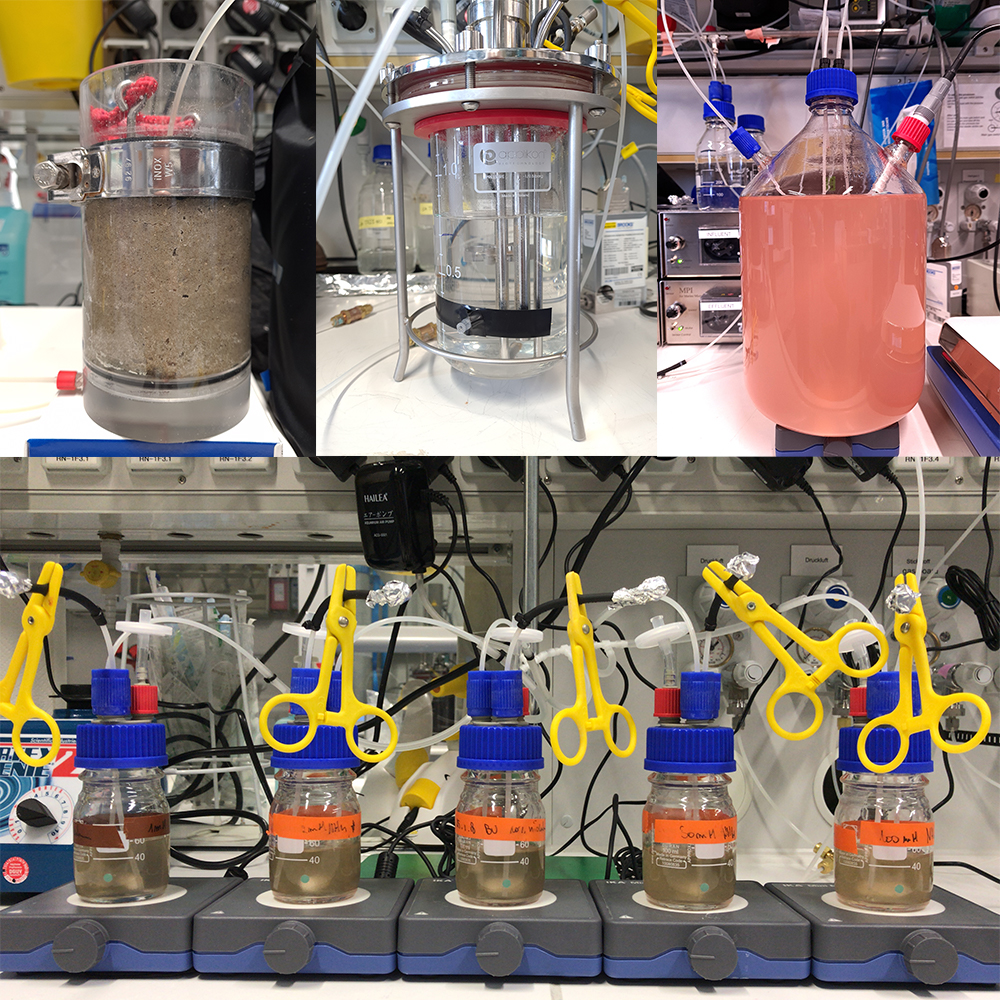
\includegraphics[scale=0.2]{Chemostat.jpg}
            \end{center}

            \normalsize{Algunas de las utilidades del quimiostato son que puede ser utilizado en cultivos puros para el estudio de la cinética del crecimiento microbiano, o para enfoques ómicos más detallados. También se puede utilizar para experimentos de competición \citep{chemostat}.}\\
            
            \normalsize{En estos experimentos se liberan en el recipiente dos o tres microorganismos diferentes, con nichos comparables en condiciones variables; con tasas de crecimiento altas o bajas; con concentraciones de oxígeno altas o bajas; distintos valores de pH o temperatura; con o sin factores de crecimiento, etc \citep{chemostat}.}

			\subsection{Ecuación de Hamilton-Jacobi.}
Desarrollamos la idea principal detr\'as de la ecuaci\'on con al que trabajaremo:\\
Sea una ecuaci\'on parcial diferencial no lineal \citep{evans} de la forma:
\begin{equation}\label{og}
	F(x;u,\nabla u)=0
\end{equation}
con $x\in\Omega\subseteq\Reals^n$, si renombramos $p\doteq\nabla u$ notaci\'on vectorial, asumimos que $F=F(x,u,p)$ es una funci\'on continua $F:\Reals^n$x$\Reals$x$\Reals^n \to \Reals$.\\
Dado $u(x)=\overline{u}(x)$ con $x\in\partial\Omega$ se construye una soluci\'on (al menos localmente, en la vecindad de la frontera) por el m\'etodo de caracter\'izticas.
Fijando un punto $x\in\partial\Omega$ consid\'erese una curva parametrizada por $t:x(t)$ con $x(0)=y$, y con:
\begin{equation*}
	\begin{split}
		u(t)&\doteq=u(x(t))\\
		p(t)&\doteq p(x(s))=\nabla u(x(t))
	\end{split}
\end{equation*}
Denotando por un punto la derivada con respecto a $t$ tenemos:
\begin{equation}\label{casi}
	\begin{split}
		\dot{u}&=\sum_i \frac{\partial u}{\partial x_i}\dot x_i=\sum_i p_i \dot x_i\\
		\dot p_j&=\sum_i \frac{\partial^2 u}{\partial x_i\partial x_j} \dot x_i
	\end{split}
\end{equation}

Diferenciando \eqref{og} con respecto a $x_j$:

\begin{equation*}
	\begin{split}
		\frac{\partial F}{\partial x_j}+\frac{\partial F}{\partial u}\frac{\partial u}{\partial x_j}+\sum_i \frac{\partial F}{\partial p_i}\frac{\partial^2 u}{\partial x_i\partial x_j}&=0\\
		-\frac{\partial F}{\partial x_j}-\frac{\partial F}{\partial u}p_j&=\sum_i \frac{\partial F}{\partial p_i}\frac{\partial^2 u}{\partial x_j\partial x_i}
	\end{split}
\end{equation*}

Al usar \eqref{casi} renombramos $\dot x_i=\frac{\partial F}{\partial p_i}$ obtenemos entonces:
\begin{equation*}
	\begin{split}
			\dot x_i&=\frac{\partial F}{\partial p_i}\\
			\dot{u}&=\sum_i p_i\frac{\partial F}{\partial p_i}\\
			\dot p_j&=-\frac{\partial F}{\partial x_j}-\frac{\partial F}{\partial u}p_j
	\end{split}
\end{equation*}
Que ahora, para un tipo espec\'ifico de problema supongamos que $F$ no depende explicitamente de $u$, entonces recuperamos las ecuaciones can\'onicas de Hamilton y podemos escribir $F\to\Ham$, y en notaci\'on vectorial.

\begin{equation*}
	\begin{split}
			\dot x&=\frac{\partial \Ham}{\partial p}\\
			\dot{u}&=p\cdot \frac{\partial \Ham}{\partial p}\\
			\dot p&=-\frac{\partial \Ham}{\partial x}
	\end{split}
\end{equation*}
con $x(0)=y$, $u(0)=u(y)$ y $p(0)=\nabla u(y)$.
De esta forma, podemos aplicar el formalismo de Hamilton-Jacobi a una variedad de problemas no necesariamente mec\'anicos, solamente pidiendo que la ecuaci\'on original cumpla $F=F(t;x,\nabla u)$.
 \subsection{Motivación para Introducir la Teoría de Hamilton-Jacobi.}
 
 En el estudio de modelos de poblaciones a trav\'es de fenotipos, ecuaciones del tipo Hamoltin-Jacobi aparecen, en especial, ecuaciones del tipo:
            \begin{equation*}
            \left\{ 
  \begin{array}{ c l }
    \frac{\partial u}{\partial t}(t,x)+b(x,I(t))\Ham (\nabla u(t,x))+R(t,x,I(t))=0 & x\in\Reals^d,t>0\\
                \min_{x\in\Reals^d} u(t,x)=0&t\geq0,
  \end{array}
\right.
            \end{equation*}

            \normalsize{\citep{Barles2006} Ecuaciones de Hamilton-Jacobi con constricciones aparecen en el estudio diversas asintósitcas singulares, es decir, situaciones en las que el comportamiento de un sistema físico o matemático cambia  de manera abrupta o presenta características extremas en ciertas condiciones, como cerca de puntos críticos, bordes o zonas donde se manifiestan discontinuidades. Estas presentan soluciones límite o aproximadas en condiciones extremas.
            }\\

            \normalsize{En los sistemas ecológicos y biológicos, la adaptación y evolución son procesos fundamentales que determinan la dinámica y supervivencia de las poblaciones. La capacidad de las especies para adaptarse a cambios en su entorno a través de la selección natural, la mutación y la competencia es un tema central en biología teórica. Para modelar estos procesos, las ecuaciones de Hamilton-Jacobi (H-J) han emergido como herramientas matemáticas poderosas para describir la evolución de poblaciones bajo distintos escenarios ecológicos.}\\

            \normalsize{\citep{Nicolas} La ecuación de Hamilton-Jacobi encuentra su aplicación en sistemas donde la dinámica de selección-mutación desempeña un papel clave. En este contexto, el cambio en el tiempo del valor de una cierta característica $\hat{s}$ en una población monomórfica, se da por medio de una ecuación de selección-mutación:}

            \begin{equation*}
                \frac{d \hat{s}}{d t}=\mu(\hat{s}) \frac{\sigma_0^2(\hat{s})}{2} n(\hat{s}) \partial_1 f(\hat{s}, \hat{s})
            \end{equation*}

            \normalsize{donde $\mu(s)$ es la probabilidad de que un nacimiento de un individuo con una característica $\hat{s}$ surja de una mutación; $\sigma_0^2(s)$ denota la varianza de distribución de una mutación $\hat{s'}$ proveniente de un individuo con característica $\hat{s}$; $\partial_1 f(\hat{s}, \hat{s}$ representa los parametros de intereacción entre individuos con característica $\hat{s}$ y $\hat{s'}$ dado por la natalidad y mortandad.}\\

            \normalsize{\citep{calvez2020} En el límite donde la tasa de mutación \( \mu \) es pequeña, las densidades de población tienden a concentrarse alrededor de valores particulares de \( x \), representando adaptaciones específicas. Este comportamiento puede analizarse mediante un ansatz de la forma:}

            \begin{equation*}
                u(x, t) \sim e^{\varphi(x, t)/\mu}
            \end{equation*}
                
            \normalsize{donde $\varphi(x,t)$ representa el frente de expansión. Sustituyendo este ansatz en la ecuación de selección-mutación y tomando el límite asintótico, se obtiene la ecuación de Hamilton-Jacobi para \( \varphi(x, t) \):}

            \begin{equation*}
                \partial_t \varphi(t, x)+H\left(I(t), x, d_x \varphi(t, x)\right)=0
            \end{equation*}
            
            }


    
    }
%-----------------------------------------------------------------
	\section{Modelo}{
				\subsection{Descripción del Entorno Biológico.}
			\normalsize{Consid\'erese un organismo con acceso a dos recursos para su supervivencia. Sean $S_1$ y $S_2$ las concentraciones de estos dos recursos contenidos en un chemostat. Entonces el vector:}
        \begin{equation}
        I=\binom{S_{1}}{S_{2}},
        \end{equation}

        \normalsize{constituye la condición ambiental para el consumidor.\citep{Diekmann2001, diekman2003}.}\\

        \normalsize{Ahora bien, estos organismos pueden especializarse de mayor o menor medida en el consumo de cualquiera de los 2 recursos a su disposici\'on. Describimos esto en un rasgo cuantizable $x$ que var\'ia continuamente entre $[0,1]$. Si $x$ equivale a 0, sólo el recurso $S_2$ es consumido, caso contrario cuando equivale 1, s\'olo se consume el recurso $S_1$. Extendiendo a escala poblacional, el impacto causado por el rasgo $x$ se toma impl\'icitamente dentro de los coeficientes $\eta(x)$ y $\xi(x)$, definidos de tal manera que la proporci\'on de ingesta \textit{per c\'apita} de un solo organismo con rasgo $x$ equivale, respectivamente a: $\eta(x)$ $S_1$ y $\xi(x)$ $S_2$.\citep{dieckman2005}}\\

        \normalsize{En el caso de una población monomórfica, la dinámica ecológica está gobernada por el siguiente sistema de ecuaciones diferenciales:}
        \begin{equation}\label{eqmono}
        \begin{split}
             \frac{d S_1}{dx}&=S_{01}-S_1-\eta(x)S_1X\\  \frac{d S_2}{dx}&=S_{02}-S_2-\xi(x)S_2X\\ \frac{d X}{dx}&=-X+\eta(x)S_1X+\xi(x)S_2X 
        \end{split}
        \end{equation}

        \normalsize{Donde X representa la densidad de la población consumidora y $S_{01}$ es la concentración del recurso i ($i\in\{1,2\}$) en el medio de entrada, para este modelo, la tasa de crecimiento poblacional de los consumidores con el rasgo $x$ bajo condiciones ambientales estables $I$ ($\frac{d X}{dx}=0$ en la tercera expresi\'on de \eqref{eqmono}), está dada por:}
        \begin{equation}\label{r}
        	\begin{split}
        			0&=r(x,I)X\\
            r(x,I)&=-1+\eta(x)S_1+\xi(x)S_2.
        	\end{split}
        \end{equation}
        
	\normalsize{Por lo tanto la primera condici\'on para estados estables es:}
				\begin{equation*}
					r(x,I)=0
				\end{equation*}
				
\normalsize{Para las 2 primeras expresiones de \eqref{eqmono} obtenemos lo siguiente para las mismas condiciones de estabilidad:}
        \begin{equation*}
        \begin{split}
             0&=S_{01}-S_1-\eta(x)S_1X\\  0&=S_{02}-S_2-\xi(x)S_2X
        \end{split}
        \end{equation*}
				\normalsize{Con la que, obteniendo $S_1$ y $S_2$ en t\'erminos de $X$ y sutituyendo en nuestra primera condici\'on de estabilidad $r=0$ tenemos:}
				
				\begin{equation*}
					-1+\frac{\eta(x)S_{01}}{1+\eta(x)X}+\frac{\xi(x)S_{02}}{1+\xi(x)X}=0
				\end{equation*}
				
        \normalsize{Que es una funci\'on mon\'otona decreciente de $X$ con l\'imite -1 para $X\to\infty$, y que tiene soluci\'on positiva para X=0 solo si:}
        \begin{equation}\label{global}
            \eta(x)S_{01}X+\xi(x)S_{02}X>1,
        \end{equation}
			\normalsize{entonces \eqref{eqmono} tiene un \'unico estado estable no trivial que es asint\'otico globalmente, dado que cumpla \eqref{global}.}

		\subsection{Sistemas de Ecuaciones de Selección-Mutación y Paso al Límite para Mutaciones.}

        \normalsize{Si la reproducción no es completamente fiel (aparece alguna mutaci\'on), un consumidor con el rasgo $y$ puede generar descendencia con el rasgo $x$. Sea $K(x,y)$ la densidad de probabilidad correspondiente. Sea $n(t,.)$ la densidad de consumidores en el tiempo t. El sistema \citep{dieckman2005}:}

        \begin{equation}\label{core}
            \begin{split}
                \frac{d S_1}{dt}(t)&=S_{01}-S_1(t)-S_1(t)\int_{0}^{1}\eta(y)n(t,x)dx,\\
               \frac{d S_1}{dt}(t)&=S_{02}-S_2(t)-S_2(t)\int_{0}^{1}\xi(x)n(t,x)dx\\
              \frac{d n}{dt}(t,x)&=-n(t,x)+\int_{0}^{1}K(x,y)[S_1(t)\eta(y)+S_2(t)\xi(x)]n(t,y)dy,
            \end{split}
        \end{equation}

        \normalsize{describe la interacción, a través de los recursos, de los diversos tipos de consumidores, así como el efecto de la mutación, le denominaremos sistema de ecuaciones de selección-mutación. Tomamos que la descendencia de un individuo con el rasgo $x$ tiene una distribución de rasgos descrita por la densidad K(x,.).}\\

        \normalsize{Adem\'as, asumiendo que las mutaciones son muy peque\~nas, de tal manera que la distribuci\'on de probabilidad $K(x,y)$ es muy peque\~no para $x$ fuera de un vecindario de radio $\varepsilon$ con ''centro'' en $y$, $\varepsilon>0$ muy peque\~no, entonces tomamos $K(x,y)\to K_{\varepsilon}(x,y)$ dependiente de este pequeño parámetro $\varepsilon$.\citep{dieckman2005}}\\

        \normalsize{Reescalamos el tiempo sustituyendo $\tau=\varepsilon$t (este escalamiento ajusta la escala temporal de modo que, al hacer $\varepsilon$ desaparecer, la escala de tiempo se adapte para observar el efecto de las mutaciones), reescribimos \eqref{core}:}

        \begin{equation}\label{nocon}
            \frac{\varepsilon}{n(\tau,x)}\frac{d n(\tau,x)}{d\tau}=-1+\int_{0}^{1}K(x,y)_{\varepsilon}[S_1(\tau)\eta(y)+S_2(\tau)\xi(x)]\frac{n(y,\tau)}{n(\tau,x)}dy.
        \end{equation}

        \normalsize{a la que a la vez podemos luego realizar la siguiente transformación}

        \begin{equation*}
            \varphi(\tau,x)=\varepsilon ln[n(\tau,x)],
        \end{equation*}
        \normalsize{entonces:}
        \begin{equation*}
            \frac{d\varphi(\tau,x) }{d\tau}=\int_{0}^{1}K_{\varepsilon}(x,y)[S_1(\tau)\eta(y)+S_2(\tau)\xi(x)]e^{\frac{\varphi(\tau,y)-\varphi(\tau,x)}{\varepsilon}}dy
        \end{equation*}

        \normalsize{Aprovechando lo mencionado anteriormente sobre $K_{\varepsilon}(x,y)$ realizamos el cambio de variable de integración $y=x+\varepsilon z$ y de la definici\'on de derivada parcial:}

        \begin{equation*}
            \frac{\varphi(\tau,y)-\varphi(\tau,x)}{\varepsilon} \to \frac{d\varphi(\tau,x) }{dx}z
        \end{equation*}

        \normalsize{y asumimos que la probabilidad de aparición de un nuevo rasgo como resultado de una mutación depende únicamente de la distancia al rasgo original. Por lo tanto, reemplazamos el kernel $K_{\varepsilon}$ por un kernel de convolución $\widetilde{K}$:}
        
        \begin{equation*}
            K_{\varepsilon}(x,y)dy\longrightarrow \widetilde{K}(z)dz
        \end{equation*}

        \normalsize{Donde $\widetilde{K}$ es una función no negativa y par definida en $(-\infty,+\infty)$, cuya integral es igual a 1. Al tomar formalmente el límite cuando $\varepsilon\to 0$ en \eqref{nocon}, obtenemos:}\\

        \begin{equation}\label{hj}
            \frac{d\varphi(t,x) }{dx}=-r(x,I)+[S_1(t)\eta(y)+S_2(t)\xi(x)]\Ham(\frac{\partial \varphi(t,x) }{\partial x})
        \end{equation}
            
        \normalsize{la ecuaci\'on de Hamilton-Jacobi, d\'onde r se define en \eqref{r} y $\Ham$ se toma como:}
        \begin{equation*}
             \Ham(p)=\int_{-\infty}^{\infty}\widetilde{K}(z)e^{-pz}dz-1
        \end{equation*}

        \normalsize{y que cumple $\Ham(0)=0$ y que, para una función par $\widetilde{K}$, $\Ham'(0)>0$; por lo tanto, $\Ham$ es convexa. Llamamos a $\Ham$ el Hamiltoniano correspondiente a $\widetilde{K}$.}   
		\subsection{Descripción Superficial del Modelo Numérico.}
   \subsection{Descripción del Método numérico}
\subsubsection{Diferencias finitas}

    Es un método numérico para la solución de ecuaciones diferenciales, se basa en la discretización de las variables dependientes e independientes convirtiendo las ecuaciones continuas en sistemas algebraicos más fáciles de resolver.

    Es una técnica útil para la solución de sistemas complejos. Consiste en aproximar las derivadas de las ecuaciones mediante \textbf{diferencias finitas}, esto es, que se reemplaza la derivada de una función en términos continuos por una expresión algebraica que involucra a la función en puntos discretos en una malla de tiempo, espacio, etc.

    \textbf{{Cómo funciona el Método de Diferencias Finitas}}
        \begin{enumerate}
            \item Discretización.

                Se discretizan las variables independientes en una malla, y las soluciones se calculan en algún punto de la malla

            \item Aproximación de Derivadas

                Las derivadas de las funciones se reemplazan por diferencias finitas en cada punto de la malla. Este reemplazo se hace dependiendo del problema

            \item Ecuaciones algebraicas

                Al reemplazar las derivadas por diferencias finitas, se obtienen ecuaciones algebraicas fáciles de resolver

            \item Iteración

                El sistema de ecuaciones se resuelve de manera iterativa, los valores de la solución en cada punto de la malla se calculan por pasos hasta obtener una solución en todo el dominio
        \end{enumerate}
        
        Este método presenta algunas ventajas y desventajas: simplicidad ya que es fácil de implementar, aplicación, es aplicable a problemas de difusión, reacción, etc. Por otro lado, tiene como inconveniente que: el error es inversamente proporcional al tamaño de la malla, pero si se hace la malla más pequeña, tiene más costo computacional, si los pasos temporales son grandes, esto puede ocasionar que la solución no sea estable\footnote{Que el método sea inestable se refiere a que el error en la solución crece conforme el tiempo}.

    \subsubsection{Diferencias finitas Semi-Implicito}

        Se usa para la solución de sistemas de ecuaciones diferenciales en los que aparecen fenómenos de difusión y reacción. Es un método que involucra la solución combinando dos métodos explicito e implícito, y el método es estable.

        \textbf{Explicito:} las variables en el paso de tiempo se calculan en el paso actual con la información del paso anterior, este es inestable en algunas ecuaciones.

        \textbf{Implicito:} las variables en el paso de tiempo se calculan en el siguiente paso, este es más costoso computacionalmente, pero es más estable

    \subsection{Aplicación a la ecuación de Selección-Mutación}
    \subsubsection{Simulación directa}

    La ecuación de Selección-Mutación \eqref{??} de forma discreta es
    \begin{equation}
        \left\{\begin{matrix}
            S_{i}^{(k+1)} = &  S_{i}^{0}-\Delta tS_{i}^{(k+1)}[1+\langle{n^{(k)}\eta_{i}}\rangle  ] \\
            n_{j}^{(k+1)} = &  n_{j}^{(k)}-\Delta t n_{j}^{(k+1)}+\Delta t([S_{1}^{(k+1)}\eta+S_{2}^{(k+1)}\xi]n^{(k)}\star \tilde{K})_{j}
        \end{matrix}\right.
    \label{eq:S-M_dis}
    \end{equation}

    donde 
    \begin{equation*}
        \langle{n^{(k)}\eta_{i}}\rangle = \frac{1}{N}\sum_{j=1}^{N}n_{j}^{(k)}\eta_{j}
    \end{equation*}

    \begin{equation*}
        (\eta n^{(k)}\star \tilde{K})_{j}=\frac{1}{2M+1}\sum_{m=-M}^{M}\eta_{j-m}n_{j-m}^{(k)}\tilde{K}_{M}
    \end{equation*}

    el primer término de la \eqref{eq:S-M_dis} representa la dinámica de los nutrientes, el segundo término se refiere a la dinámica de los consumidores, $\langle{n^{(k)}\eta_{i}}\rangle$ es el promedio de la densidad de consumidores por su capacidad de consumir uno de los nutrientes, y $(\eta n^{(k)}\star \tilde{K})_{j}$ es la operación de convolución, este modula las interacciones de los consumidores en el espacio discreto del rasgo $x$, $y$

    \subsubsection{Aproximación Hamilton-Jacobi}

    

	}
%-----------------------------------------------------------------
	\section{Conclusiones y Comentarios Finales}
	\clearpage
%---------------------------------------------------------------
	\bibliographystyle{plain}
	\bibliography{referencias.bib}
%------------------------------------------------
\end{document}
